\section{Related Work}\label{sec:related}

SoundCode sits at the intersection of three lines of work:
(i) decoding-time methods that consult a programming-language
verifier and react to its output --- the closest neighbours, treated
in detail below; (ii) per-token constrained-decoding methods that
mask the LM's logit vector against a grammar or type lattice but do
not roll back; and (iii) speculative-decoding methods that run a
verifier asynchronously alongside the LM, but use the LM itself as
the verifier. SoundCode borrows the rollback algorithm from (i), the
mask-when-cheap idea from (ii), and the parallel-verify control flow
from (iii); its open contribution is to combine all three.

\subsection{Verifier-in-the-loop decoding (the closest neighbours)}
\label{sec:rw-direct}

\paragraph{Monitor-Guided Decoding (MGD).}
\citet{agrawal2023monitor} introduce a framework in which a
stateful \emph{monitor} sits between the LM and a Language Server
Protocol (LSP) instance. The monitor's pre-condition fires on a
trigger token (in the canonical instantiation, the \code{.} that
begins a Java member-access expression). On firing, the LSP returns
the type-consistent identifiers reachable at that source location;
the monitor converts the set to a binary mask over the LM
vocabulary, zeroes the logits of tokens not prefixing any allowed
identifier, and resumes decoding. Each tokenization step that lands
on a trigger pays a synchronous LSP round-trip. The reported
mean-decoding-time slowdown is approximately
$83\%$ \citep[Table 2]{agrawal2023monitor} on Java
DOTPROMPTS, traded for a $+18\%$ to $+25\%$ relative compilation-rate
gain across CodeGen-350M to text-davinci-003. The monitor does not
roll back: if a triggered LSP query returns an empty allowed set,
the run is abandoned. MGD is the canonical \emph{prevention by
masking} design point.

\begin{figure}[t]
  \centering
  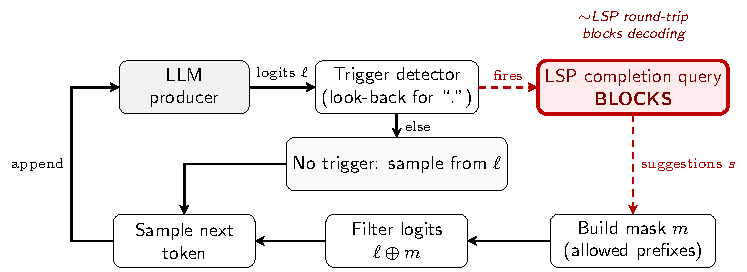
\includegraphics[width=0.78\linewidth]{figures/mgd_workflow.pdf}
  \caption{Monitor-Guided Decoding \citep{agrawal2023monitor}: the
    LSP is queried at each trigger token (\code{.} in Java); tokens
    outside the returned suggestion set are masked to $-\infty$. The
    LSP round-trip blocks decoding at every triggered token.}
  \label{fig:mgd-workflow}
\end{figure}

\paragraph{ROCODE.}
\citet{jiang2024rocode} compile-check after every emitted statement,
roll back on a detected error, and decode the retry under an
exponentially-decaying token-penalty mask. Two rollback rules
coexist: $r_e$, the error-line offset reported by the compiler, is
tried first; if the compiler error recurs at the same line, the
system falls back to $r_h$, the line containing the highest-entropy
token in the prefix
\citep[Eqs.~5--7]{jiang2024rocode}. A Trie tracks attempted
paths so previously-failed token suffixes accumulate decayed
penalties on each retry. ROCODE targets Python and C++ and reports a
PassRate of 57.3 on HumanEval(ET) with CodeLlama-7B at
$p\!=\!0.9$ nucleus, $+30.6$\,pp over the unconstrained baseline and
$+11.0$\,pp over PG-TD. Crucially, the verifier runs
synchronously between statements; the design only works because
Python's \code{compile()} returns in $\sim$0.1\,ms and
$g{+}{+}\;\code{-fsyntax-only}$ in $\sim$3\,ms.
ROCODE is the closest direct competitor to SoundCode.

\begin{figure}[t]
  \centering
  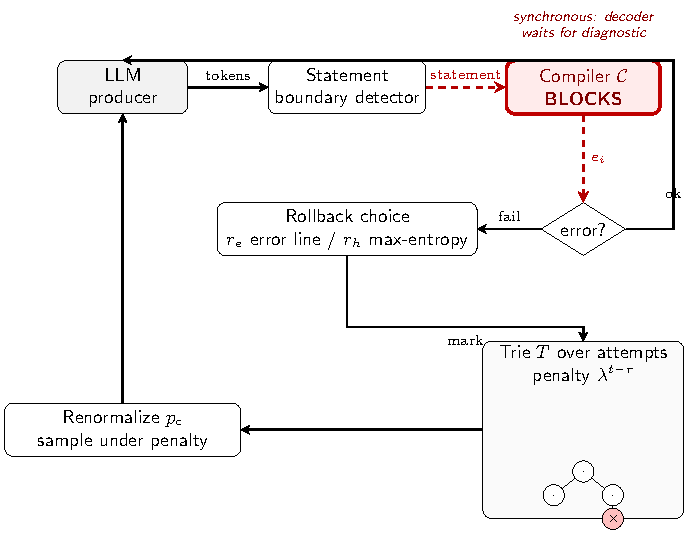
\includegraphics[width=0.78\linewidth]{figures/rocode_workflow.pdf}
  \caption{ROCODE \citep{jiang2024rocode}: the compiler runs
    synchronously after each emitted statement; on a detected error,
    the buffer is rolled back to the compiler-reported line, or, on
    recurrence, to the line containing the highest-entropy token.
    The retry decodes under an exponentially-decaying token-penalty
    mask.}
  \label{fig:rocode-workflow}
\end{figure}

\paragraph{SemGuard.}
\citet{wang2025semguard} train a 1.3B LLM-based binary classifier on
a curated diff corpus (SemDiff) that pairs correct and incorrect
submissions to the same problem from CodeNet. After every emitted
line, the classifier scores the partial program; if the score drops
below 0.5, the LM rolls back to the start of the line and resamples
under a single-token penalty on the offending first non-indent
token, retrying up to $N$ times. SemGuard targets Python and Java
and reports a $+2.23$\,pp gain over ROCODE on SemDiff with
DeepSeek-Coder-6.7B, at 31\% fewer tokens and 60\% lower wall-clock
\citep[Tables 3, 6]{wang2025semguard}.
The verifier is again synchronous, but the per-line classifier-pass
cost (single-digit ms on a modern GPU) is comparable to ROCODE's
\code{compile()}-based version. The verifier is \emph{learned}, so
soundness is empirical rather than guaranteed --- SemGuard reports
per-task false-positive rates centred on 0.26--0.34.

\begin{figure}[t]
  \centering
  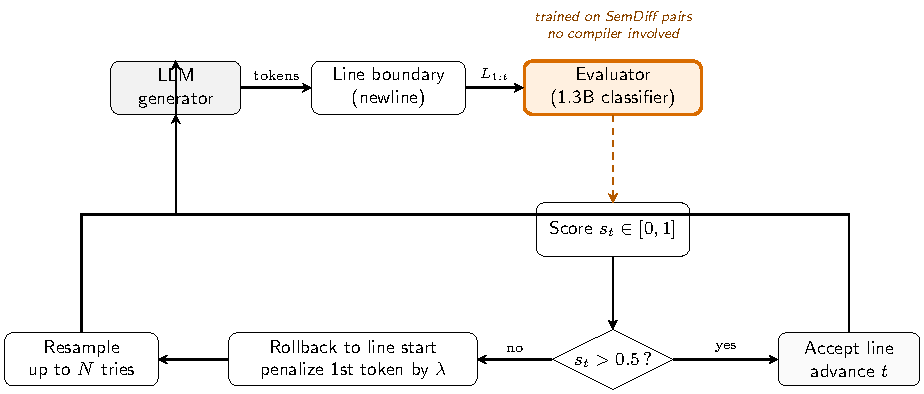
\includegraphics[width=0.78\linewidth]{figures/semguard_workflow.pdf}
  \caption{SemGuard \citep{wang2025semguard}: a learned 1.3B
    semantic classifier scores each emitted line; if the score
    drops below 0.5, the buffer is rolled back to the start of the
    offending line and the LM resamples under a single-token
    penalty on the first non-indent token, up to $N$ retries.}
  \label{fig:semguard-workflow}
\end{figure}

\paragraph{IterGen.}
\citet{ugare2025itergen} target grammar-constrained structured-output
generation (SQL, Vega-Lite JSON, regex). They expose a Python API of
\code{forward(symbol, n)}, \code{backward(symbol, n)}, and
\code{view(symbol)} primitives indexed by grammar non-terminals, and
implement backward via KV-cache cropping driven by a shift-reduce
parser's symbol-position map. The verifier is whatever Python
predicate the user writes against \code{view(symbol)} --- typically a
schema-membership check, a regex match, or a JSON field-type
assertion. Verification is synchronous between \code{forward} calls
but cheap because the user predicates are typically constant-time.
SoundCode borrows IterGen's KV-cropping idea as a low-overhead
rollback implementation; the verifier differs (real compiler vs.\
user predicate) and the target language differs (Turing-complete
Rust vs.\ declarative DSLs).

\subsection{Constrained decoding without rollback}\label{sec:rw-cd}

A separate line of work prevents bad outputs by masking the LM's
logits against a grammar, type lattice, or completion engine, but
never rolls back: rejected tokens never make it into the buffer in
the first place. \emph{PICARD} \citep{scholak2021picard} runs a
fast monadic SQL parser on each top-$k$ beam continuation and
assigns $-\infty$ to tokens whose partial detokenization fails to
parse; \emph{Synchromesh} \citep{poesia2022synchromesh} generalizes
this with hand-written Completion Engines for SQL, Vega-Lite, and
SMCalFlow, using Brzozowski derivatives to reconcile LM-token vs.\
DSL-token mismatch. \emph{Grammar-Constrained Decoding}
\citep{geng2023gcd} extends the mask to arbitrary
context-free grammars; \emph{DOMINO} \citep{beurerkellner2024domino}
makes the mask near-zero-overhead via per-state prefix trees and
opportunistic argmax-first verification.
\emph{Type-Constrained Code Generation}
\citep{mundler2025typeconstrained} extends the construction from
syntax to types: a prefix automaton plus a type-reachability search
enforce well-typedness of every sampled token on a simply-typed
Turing-complete calculus, implemented for TypeScript. The reported
median per-instance overhead is $39$--$52\%$; pass@1 rises by
$+3.5\%$--$+5.0\%$ on TypeScript HumanEval and MBPP synthesis.
All of these systems are synchronous and per-token, and none rolls
back; semantic errors that surface only across multiple tokens
(borrow-checker violations, multi-statement type-inference failures)
are out of reach for them by construction. They are most useful as
\emph{cheap front-ends} composed with SoundCode's
expensive-verifier-with-rollback back-end.

\subsection{Speculative decoding: the structural blueprint}\label{sec:rw-spec}

The structural insight SoundCode reuses is the
\emph{speculate-ahead, verify-in-parallel, accept-or-rollback}
control flow of speculative decoding. \citet{leviathan2023speculative}
and \citet{chen2023speculative} draft $K$ tokens from a small fast
model, then score them in a single parallel forward pass of the
large target model, accepting a left-to-right prefix while
provably preserving the target distribution. Reported speedups are
$2.46\times$ on HumanEval with Chinchilla 70B
\citep{chen2023speculative} and up to $3.4\times$ on translation
\citep{leviathan2023speculative}. \citet{fu2024lookahead} achieve a
draft-model-free variant by reformulating decoding as a Jacobi
fixed-point and verifying cached $n$-grams in parallel inside the
same model, reaching $1.5\times$--$2.3\times$ on a single A100 and
up to $4\times$ with Lookahead Parallelism on 8 A100s.
SoundCode swaps the LM-as-verifier for a \emph{semantic} verifier
(\code{cargo check} + LSP) and replaces per-token rollback with
structural-boundary rollback. The control-flow skeleton --- producer
runs ahead, verifier runs in parallel, on rejection rollback to a
prior accept --- is the same.

\subsection{Iterative repair (the contrast)}\label{sec:rw-repair}

A sibling family runs the verifier \emph{off} the critical path
entirely. Self-Refine \citep{madaan2023selfrefine},
Reflexion \citep{shinn2023reflexion}, Self-Debug
\citep{chen2024selfdebug}, INTERVENOR \citep{wang2024intervenor}, and
AlphaCodium \citep{ridnik2024alphacodium} all generate a whole
candidate solution, run the verifier on the finished artifact, and
condition a fresh generation on the verifier's natural-language
output. These pay for the verifier only once per solution but
discard a long completion on each fix attempt. The pivotal
methodological result is \citet{olausson2024selfrepair}'s observation
that, across HumanEval and APPS, self-repair beats matched-budget
i.i.d.\ resampling only when the feedback model is \emph{strictly
stronger} than the generator --- a same-model self-critique loop
roughly cancels its own compute cost.
SoundCode is designed to clear this bar: \code{cargo check} is
strictly stronger than the generator on the decidable fragment of
syntax, type, and lifetime correctness.

\subsection{Benchmarks and base models}\label{sec:rw-bench}

We evaluate on MultiPL-E HumanEval-rs and HumanEval-cpp
\citep{cassano2022multipl}, two of the multilingual ports of the
original HumanEval benchmark \citep{chen2021humaneval}; the source
problems are 164 hand-written Python signatures plus docstrings,
mechanically translated to Rust and C++ with native-language unit
tests preserved. The base model is Qwen2.5-Coder-7B-Instruct
\citep{hui2024qwen25coder}, a frontier open-weight code LM in the
7B class.

\subsection{Synthesis}\label{sec:rw-synth}

The four-way SoundCode framing follows from the survey: every
decoding-time-with-verifier system in
Section~\ref{sec:rw-direct} runs synchronously; every async
parallel-verify system in Section~\ref{sec:rw-spec} uses the LM as
verifier. The combination semantic-verifier $\times$
structural-rollback $\times$ asynchronous-on-the-critical-path is the
open design point. The choice of verifier (real compiler / LSP vs.\
learned classifier vs.\ grammar) is forced once one commits to that
combination: a learned classifier is too weak by Olausson's
criterion; a grammar is too weak for type and borrow correctness; a
compiler is strong enough, but its latency makes synchronous use
impractical, so the async design is what unlocks the use of the
strictly-stronger oracle.
